\section*{Схема экспериментальной установки}

Схема экспериментальной установки изображена на рисунке:

\begin{figure}[H]
	\centering
	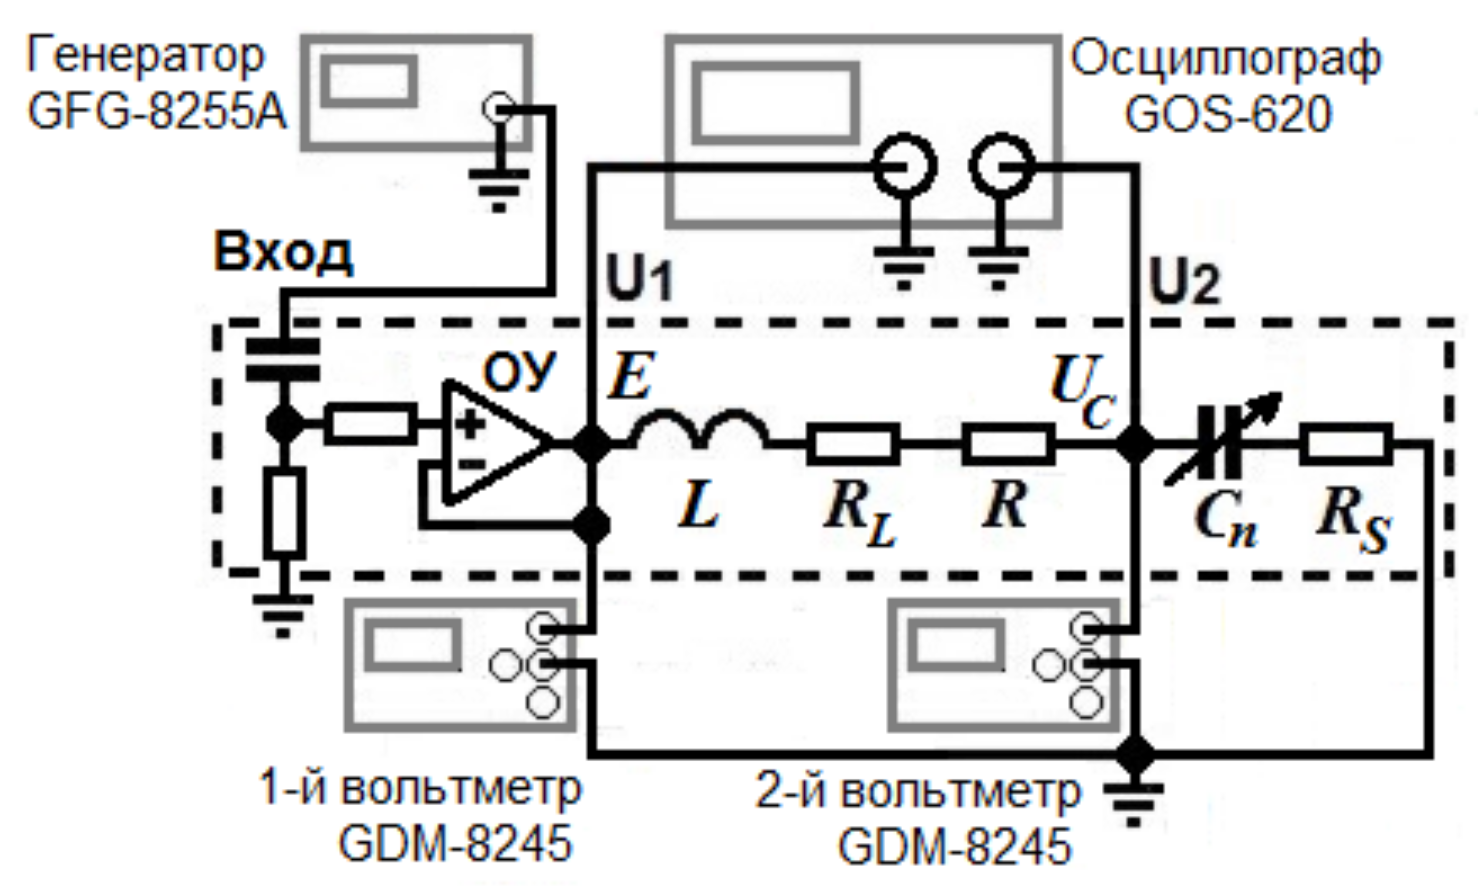
\includegraphics[width=0.5\textwidth]{../res/exp_scheme.png}
\end{figure}

Генератор синусоидального сигнала подключается к схеме через усилитель. Напряжение на входе и конденсаторе измеряется вольтметрами и осциллографом. Предполагается, что индуктивность и емкость обладают активным сопротивлением, которое учитывается резисторами $R_L$ и $R_S$.

В работе исследуются амплитудно- и фазо- частотные характеристики данной схемы.